\documentclass[10pt,a4paper]{article}
\usepackage[utf8]{inputenc}
\usepackage[a4paper, total={6in, 8in}]{geometry}
\usepackage{graphicx}
\usepackage{subcaption}
\usepackage{float}
\begin{document}
\begin{titlepage}
\begin{center}
\newcommand{\HRule}{\rule{\linewidth}{0.5mm}}
% Upper part of the page. The '~' is needed because \\
% only works if a paragraph has started.

\includegraphics[width=0.15\textwidth]{./SwanseaLogo}~\\[1cm]

\textsc{\LARGE University of Swansea}\\[1.5cm]

\textsc{\Large Project Report 2}\\[0.5cm]

% Title
\HRule \\[0.4cm]
{ \huge \bfseries Project Report 2\\ April $22^{nd}$ 2015 \\[0.4cm] }

\HRule \\[1.5cm]

% Author and supervisor
\noindent
\begin{minipage}{0.4\textwidth}
\begin{flushleft} \large
\emph{Author:}\\
Robert \textsc{James}
\end{flushleft}
\end{minipage}%
\begin{minipage}{0.4\textwidth}
\begin{flushright} \large
\emph{Supervisor:} \\
Professor Biagio \textsc{Lucini}
\end{flushright}
\end{minipage}

\vfill

% Bottom of the page

\end{center}

\clearpage

\end{titlepage}


\section{Goals}
To this point, the primary focus has been to construct a generalised Potts model simulation in 2D that replicates the results of others strewn about the internet.
Due to the nature of the model in use, it is hard to find experimental data that has behaviour similar to that which we expect. It has become apparent that the first goal I should achieve is comparison of my results against a non generalised q so I can verify that the results are correct.

\section{Progress Made}

\subsection{$q=2$ $d=2$ Potts/Ising Model}
\begin{figure}[H]
\centering
	\begin{subfigure}[b]{0.4\textwidth}
		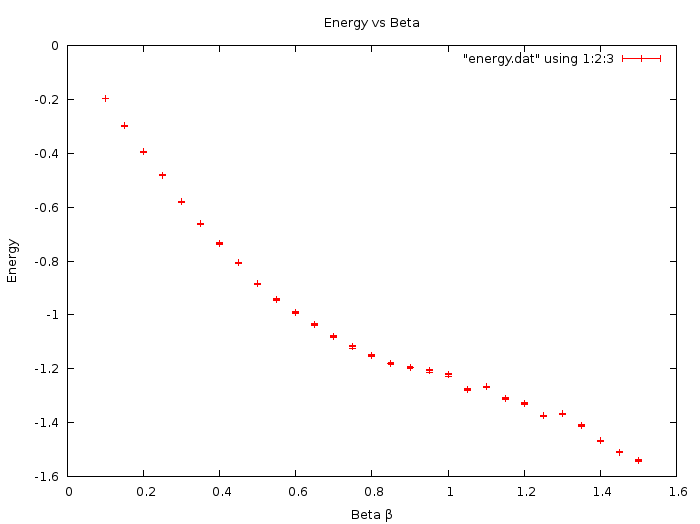
\includegraphics[width=\textwidth]{energyvsbeta.png}	
		\caption{Energy per Lattice Site}
	\end{subfigure}
	%
	\begin{subfigure}[b]{0.4\textwidth}
		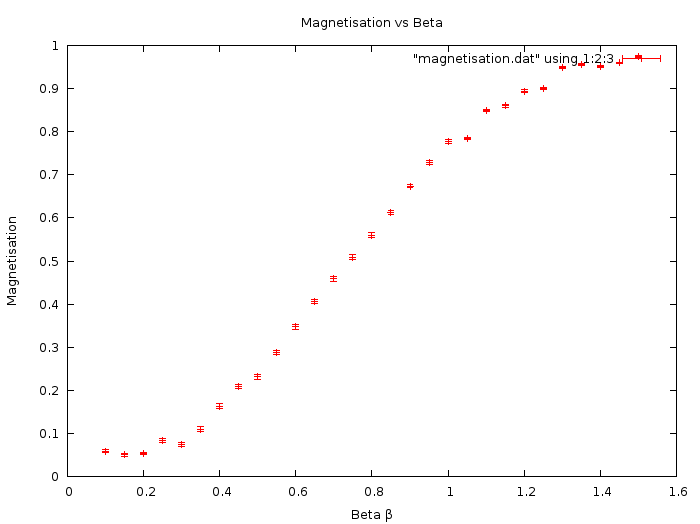
\includegraphics[width=\textwidth]{magnetisationvsbeta.png}
		\caption{Magnetisation per Lattice Site}
	\end{subfigure}

\caption{Plots of both taken on lattice size $15 \textrm{x} 15$}
\end{figure}
In the above plots it is important to remember that for $\beta$ small, $T$ is large.
So for the Energy, at small $\beta$ you get a growth in the Energy as you would expect because $T \propto E$.
At large $\beta$,$i.e./ T$ small you find that the energy returns to the minimum expected value.

In the magnetisation plot the results are as expected.
Spontaneous magnetisation doesn't exist above the critical temperature\cite{Montroll1963} so for $\beta$ small you find values around $0$.
Due to the nature of the simulation, it is difficult to achieve the exact solution provided by Osanger\cite{Montroll1963} because of perturbations performed on the system.
At low T, high $\beta$ we can see spontaneous magnetisation occurs.
Both of the plots show a transition in a similar location.
Taking the Magnetisation data into a piece of fitting software, OriginPro we can plot the smoothed $2^{nd}$ derivative of the data to extract the exact value of the phase transition.
\begin{figure}[H]
\centering
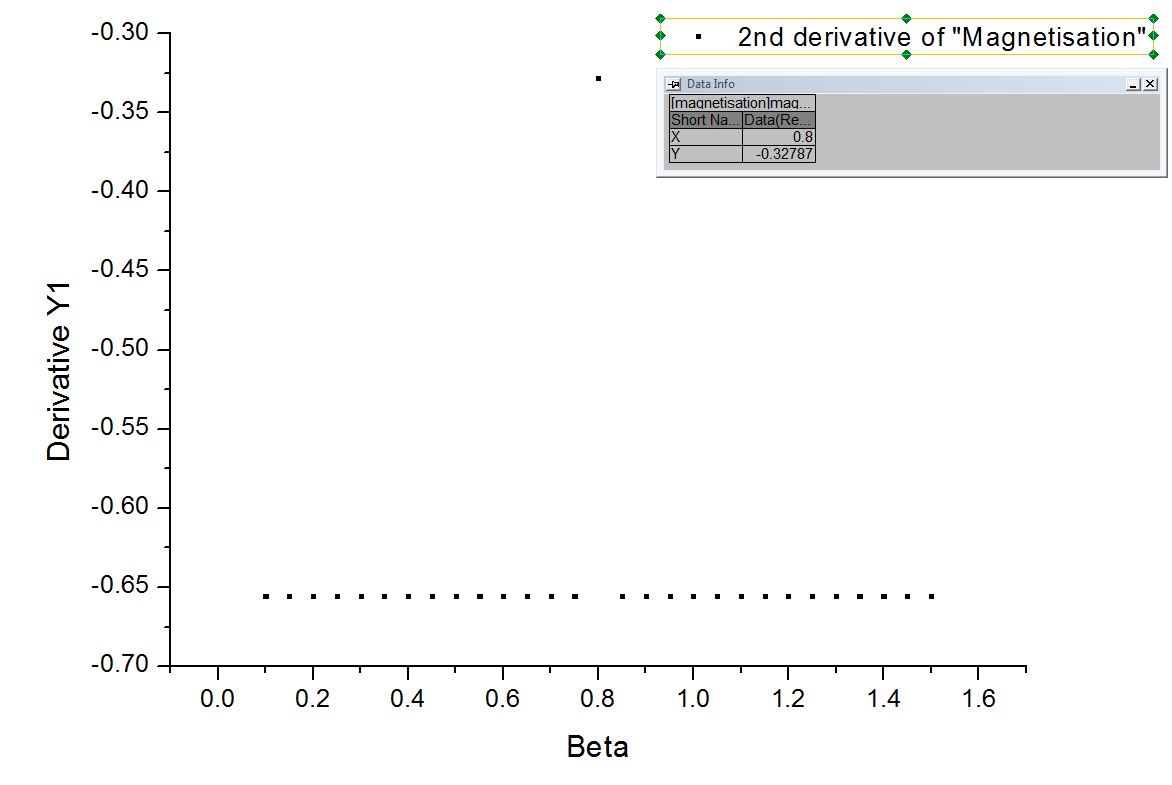
\includegraphics[width=0.5\textwidth]{2ndDerivativeMagnetisation.PNG}
\caption{Plot of the 2nd Derivative of the Magnetisation}
\end{figure}
From this we can easily see a phase transition occurring at $\beta = 0.8$.

\subsection{$q=3/4$ $d=2$ Potts Model}
The plots below reveal some interesting data for $q=3$. 
This behaviour is erratic and unexpected, therefore I am currently treating it as an error in my simulations. (therefore it is being treated as erroneous within the current simulations.) 
For $q=4$ we have similar behaviour to q=2 but with a modified transition $\beta$.
This seems to be the correct behaviour for $q=4$.
\begin{figure}[H]
\centering
	\begin{subfigure}[b]{0.4\textwidth}
		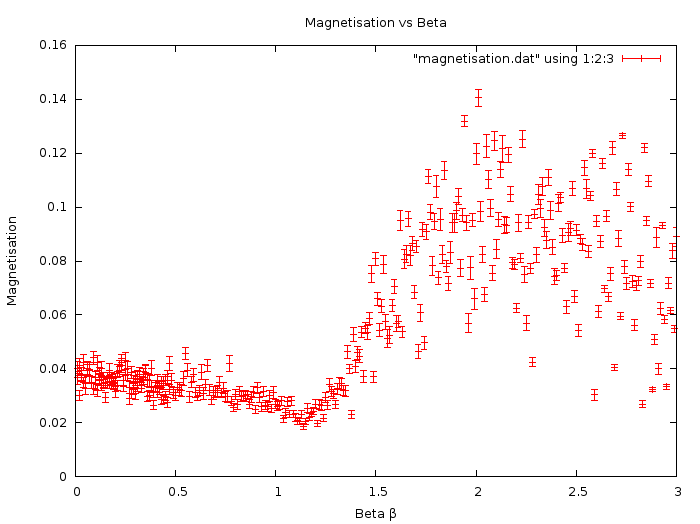
\includegraphics[width=\textwidth]{q=3magnetisationvsbeta.png}	
		\caption{Magnetisation q=3 per Lattice Site}
	\end{subfigure}
	%
	\begin{subfigure}[b]{0.4\textwidth}
		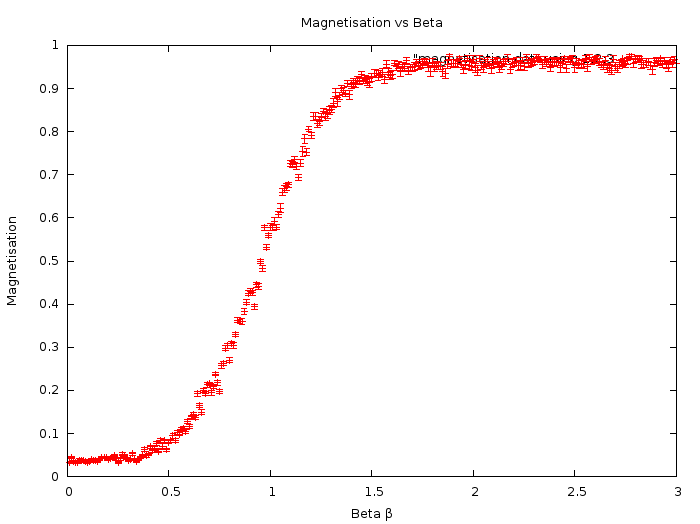
\includegraphics[width=\textwidth]{q=4magnetisationvsbeta.png}
		\caption{Magnetisation q=4 per Lattice Site}
	\end{subfigure}
\caption{Plots of both taken on lattice size $15 \textrm{x} 15$}
\end{figure}
In the plots below, there is some interesting behaviour particularly in the $q=4$ case.
The system seems to form a metastable state while the temperature is varied across the phase transition.
\begin{figure}[H]
\centering
	\begin{subfigure}[b]{0.4\textwidth}
		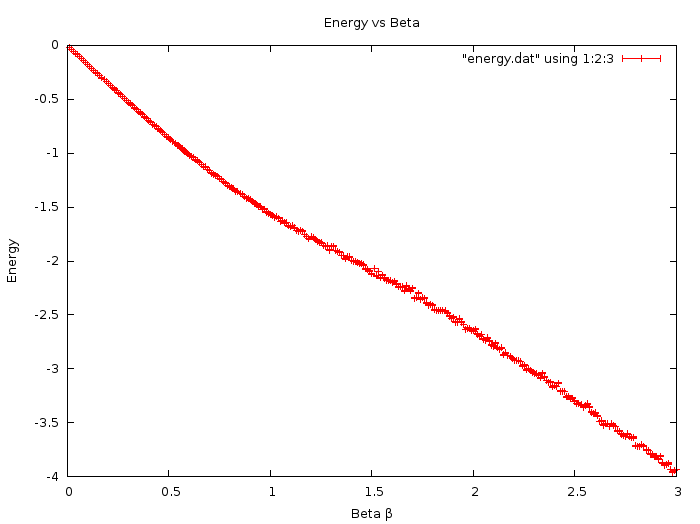
\includegraphics[width=\textwidth]{q=3energyvsbeta.png}	
		\caption{Energy q=3 per Lattice Site}
	\end{subfigure}
	%
	\begin{subfigure}[b]{0.4\textwidth}
		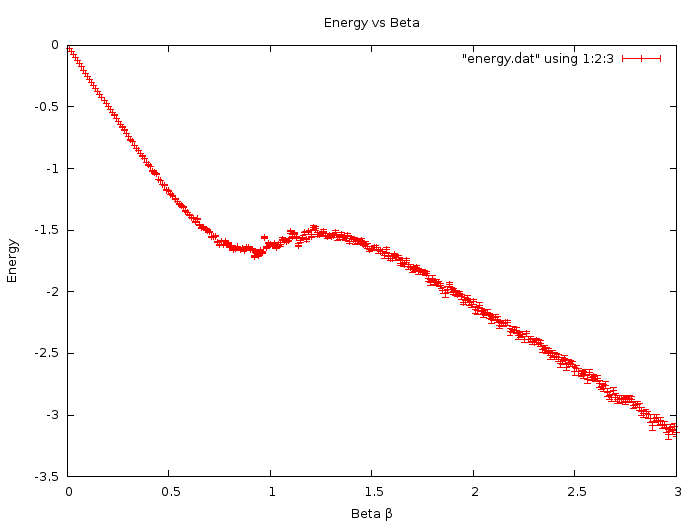
\includegraphics[width=\textwidth]{q=4energyvsbeta.png}
		\caption{Energy q=4 per Lattice Site}
	\end{subfigure}

\caption{Plots of both taken on lattice size $15 \textrm{x} 15$}
\end{figure}
In the plots below we have the $1st$ and $2nd$ smoothed derivatives of the magnetisation to allow us to study the phase transition.
In this model we are studying a $2nd$ order phase transition and we can clearly see a discontinuous function describing both $q=3 and q=4$ behaviour.
This backs up the idea that we are working with a second order phase transition.
\begin{figure}[H]
\centering
	\begin{subfigure}[b]{0.4\textwidth}
		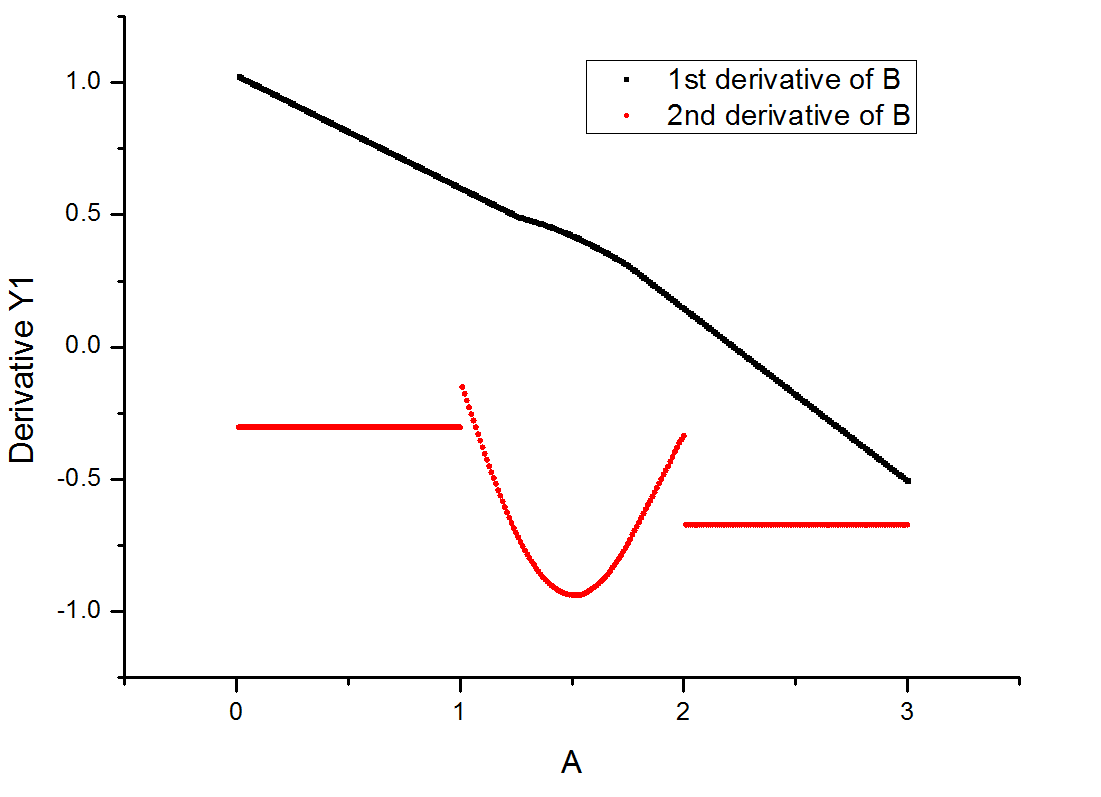
\includegraphics[width=\textwidth]{q=4magnetisationderivatives.PNG}	
		\caption{$1^{st} and 2^{nd}$ Derivatives of the Magnetisation q=3 per Lattice Site}
	\end{subfigure}
	%
	\begin{subfigure}[b]{0.4\textwidth}
		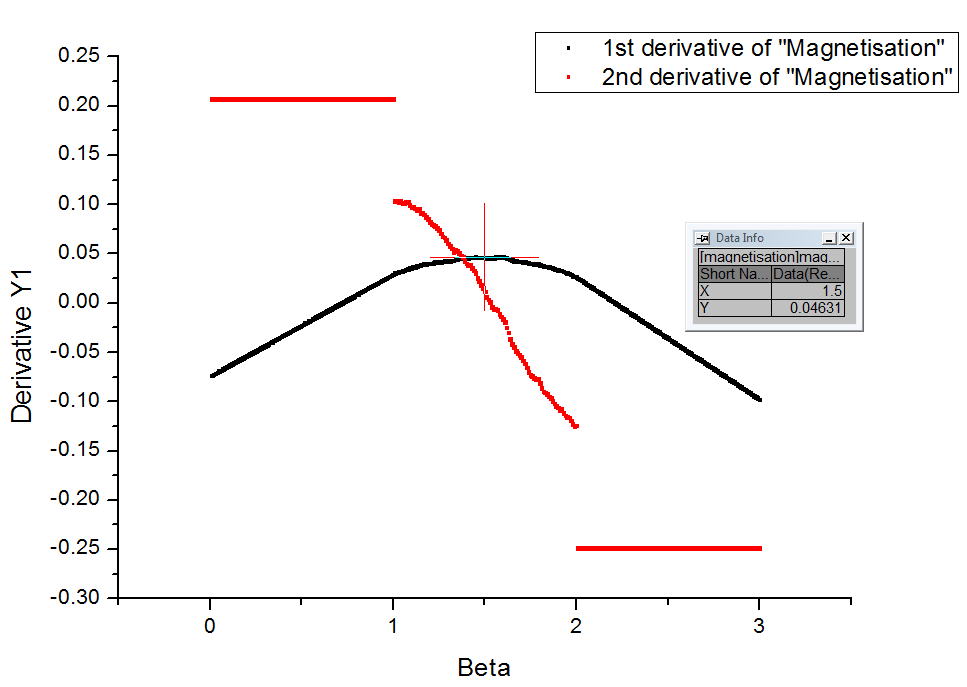
\includegraphics[width=\textwidth]{q=3magnetisationderivatives.PNG}
		\caption{$1^{st} and 2^{nd}$ Derivatives of the Magnetisation q=4 per Lattice Site}
	\end{subfigure}
\caption{Plots of both taken on lattice size $15 \textrm{x} 15$}
\end{figure}
\section{Future Plans}
Now the focus of research turns to implementing the Wang Landau algorithm and from there progressing onto interface tensions.
By reading a 2012 paper by M Guagnelli on using/implementing the Wang-Landau algorithm and comparing his test case results for $d=2$ $q=10$, further understanding of the method as a whole and hopefully future insight as to the direction of the project will be gained.

Ongoing optimisation of the update algorithm will be required upto and beyond the implementation of interface tensions to ensure optimum run times.  
Because the next stage in work requires sampling from a target energy band, the code already has a modified version of the Heat Bath algorithm that can drive a system towards a target energy.
To be sampling on/around the critical temperature for the next stage of the research, further calculations of $\beta$ will be required.
Calculating $\beta$ values for various grid sizes allows a prediction of $\beta$ at the thermodynamic limit $\lim_{N \to \infty}$.

Adding other thermodynamic quantities such as the Specific Heat $C_{V}$ and the Magnetic Susceptibility $\chi$ to program output will significantly improve the academic value of any future research.

\bibliographystyle{plain}
\bibliography{References}

\end{document}
